%% Template for MLP Coursework 1 / 16 October 2017 

%% Based on  LaTeX template for ICML 2017 - example_paper.tex at 
%%  https://2017.icml.cc/Conferences/2017/StyleAuthorInstructions

\documentclass{article}

\usepackage[T1]{fontenc}
\usepackage{amssymb,amsmath}
\usepackage{txfonts}
\usepackage{microtype}
\usepackage{enumitem}

\usepackage[utf8]{inputenc}
\usepackage{csquotes}

% For figures
\usepackage{graphicx}
\usepackage{subfigure} 

% For citations
\usepackage{natbib}

% For algorithms
\usepackage{algorithm}
\usepackage{algorithmic}

% the hyperref package is used to produce hyperlinks in the
% resulting PDF.  If this breaks your system, please commend out the
% following usepackage line and replace \usepackage{mlp2017} with
% \usepackage[nohyperref]{mlp2017} below.
\usepackage{hyperref}
\usepackage{url}
\urlstyle{same}

% Packages hyperref and algorithmic misbehave sometimes.  We can fix
% this with the following command.
\newcommand{\theHalgorithm}{\arabic{algorithm}}


% Set up MLP coursework style (based on ICML style)
\usepackage{mlp2017}
\mlptitlerunning{MLP Coursework 4 (\studentNumber)}
\bibliographystyle{icml2017}

\DeclareMathOperator{\softmax}{softmax}
\DeclareMathOperator{\sigmoid}{sigmoid}
\DeclareMathOperator{\sgn}{sgn}
\DeclareMathOperator{\relu}{relu}
\DeclareMathOperator{\lrelu}{lrelu}
\DeclareMathOperator{\elu}{elu}
\DeclareMathOperator{\selu}{selu}
\DeclareMathOperator{\maxout}{maxout}

%% You probably do not need to change anything above this comment

%% REPLACE this with your student number
\def\studentNumber{s1700260, s1457374, s1784849}

\begin{document} 

\twocolumn[
\mlptitle{MLP Coursework 4: Project Final Report \\
Transfer learning and dataset size\\
Group G74
}

\centerline{\studentNumber}

\vskip 7mm
]

\begin{abstract} 
Write This Last.
\end{abstract} 

\section{Introduction}
\label{sec:intro}

Large-scale neural networks have become increasingly prevalent in artificial intelligence \cite{krizhevsky2012imagenet}. Such architectures effectively solve computer vision problems that were previously considered difficult to address using traditional symbolic manipulation \cite{dinsmore2014symbolic}. One concern with modern neural networks is that their performance scales with the quantity of data used to train them, as demonstrated in our previous piece of research \cite{interim-report}. This concern is a problem for individuals or institutions with small amounts of data that want to implement these architectures as solutions, or for research purposes.

Data driven techniques exist, such as data augmentation \cite{krizhevsky2012imagenet}, which help solve this problem\footnote{see our previous paper for a further explanation.}. However, to draw from our previous research \cite{interim-report} we investigate alternative, machine learning based approaches, specifically transfer learning \cite{oquab2014learning}, \citep{ng2015deep} and deep features extraction \citep{chen2016deep} as methods to improve the performance of neural network architectures that utilise small amounts of data. These techniques allow us to use the knowledge that a given (pre-trained) network already has and adapt the architecture to suit our requirements.

The objective of transfer learning is to use the knowledge acquired by an existing network that was built to solve a similar task and improve the generalization. The main idea is to try to adapt that previous knowledge to the new problem to be solved. One of the advantages of this technique is that the solution for the new problem does not have to start from scratch. Prior work can be re-utilised which is important when the resources are limited. This situation is specially true for convolutional neural networks which, depending on the size of the architecture, can require an important amount of computational power.

There exist a number of pre-trained neural networks to solve classification tasks in the field of computer vision. One of them is the Visual Geometry Group network (VGG net) \cite{DBLP:journals/corr/SimonyanZ14a}. This network implements a simple yet deep architecture with several convolutional layers. There are several configurations that vary the number of convolutional layers among 11, 13, 16, and 19. In every configuration the architecture includes maximum pooling layers of dimensions 2x2 and stride 1. The convolutions are performed using 3x3 filters with stride and pad of 1. Finally, ReLU activations after each convolution are utilised.

VGG net was first used in the ImageNet Challenge 2014 \cite{DBLP:journals/corr/SimonyanZ14a}, which means that is was originally trained using the Imagenet dataset \cite{deng2009imagenet}. However, the network has also been trained in other datasets like CIFAR-10 \cite{krizhevsky2014cifar} and CIFAR-100 \cite{CIFAR-100}. It is important to make this distinction since each dataset has been developed for a different purpose, therefore, they have specific characteristics. The knowledge learnt from a network depends on the dataset used to train it. Thus, it is critical to know the characteristics of the dataset utilised to train the network since it will play and important role when implementing transfer learning.

ImageNet is a large-scale hierarchical image database \cite{ImageNet}. The structure of this dataset contains 12 main groups or sub-trees. Each sub-tree contains a variable number of categories. The total number of categories is 5247, each one containing on average 600 images; thus, the total number of images in the dataset is 3.2 million. As described, ImageNet is a large and diverse dataset. However, the original version of VGG net was trained on a subset of Imagenet that contains only 1000 categories using 1.3 million images for training, 50K images for validation and 100K images for testing.

\subsection{Interim Report Findings}
\label{sec:findings}

The research questions offered within this report have been drawn from our initial findings, as documented in the interim report \cite{interim-report}. To aid in orientating the reader, we provide a summary of these findings here.

It was possible to demonstrate how the amount of available data impacts the performance of a convolutional neural network. Such impact was observed in the validation stage by analysing the accuracy and error of the network. In the first case, it was evident the reduction of the accuracy as the size of the dataset was reduced. In the second case, the size of the dataset directly affected the error; the smaller the dataset, the bigger the error. In both cases, the ultimate effect of such behaviour was the difficulty of the network to generalize when the amount of data is small.

Futhermore, the usage of two different but comparable databases provided some extra insights about the behaviour of the neural network. In this case the observed accuracies in the validation stage were different for each dataset in every size used to train the network. Under these circumstances, it was clear that the dataset that allowed a higher accuracy (clothes) was less challenging for the network. This means, that the features extracted by the network were more useful and relevant for one of the datasets. In the other hand, the features learned by the network did not provide enough information to reach better results for the second dataset (expressions).

Finally, we demonstrated that a simple data driven technique like data augmentation effectively improves the performance of a simple convolutional neural network. However, the benefits of this method have a limit above which no further improvement can be done. All of these findings provided the foundations and motivation for our investigation.

\section{Objectives and Research Questions}
\label{sec:obj_questions}

\subsection{Objectives}
\label{sec:objectives}

The research presented within this report pertains to two fundamental objectives. The first one concerns with improving the performance of image classification tasks using transfer learning with limited amounts of data. The second objective investigates the generalisability of the methods as mentioned above to two distinctly different datasets. Furthermore, we intend to propose and utilise a framework for measuring the similarity between datasets using a modified siamese neural network \cite{koch} architecture.

\subsection{Research Questions}
\label{sec:questions}

Following from the conclusions drawn from our interim report, our research questions are listed below.

\begin{enumerate}
  \item How much the performance for a given classification task can be improved by using transfer learning?  
  \item How much the application of transfer learning affect two distinct but comparable datasets?
\end{enumerate}

\subsection{Hypotheses}
\label{sec:hypotheses}
\begin{enumerate}[label=\textbf{H.\arabic*}]
  \item \label{h:1} Transfer learning will provide a performance benefit with respect to the generalisability (measured through validation accuracy) for a given classification with small data.
  \item \label{h:2} Transfer learning will provide a larger performance boost when the size of the dataset used to initially train the model is small rather than large.
\end{enumerate}

Within the remainder of this report a section that outlines the methodologies utilised to conduct our research \ref{sec:methodology} is initially given. Thereafter, all experimental results are presented \ref{sec:experiments} and a review of related work is provided \ref{sec:related}. Finally, a set of conclusions are drawn \ref{sec:conclusions}.

\section{Methodology}
\label{sec:methodology}

\subsection{Simple Transfer Learning}
\label{sec:transferlearninng}

\subsubsection{\textbf{Chosen Model}}

We decided to select the VGG net configuration with 16 convolutional layers (hereinafter referred as VGG16) to transfer its knowledge into the clothes and expressions datasets. As previously mentioned, this network is quite simple and deep, thus, the expectation is that the knowledge contained in this network will be sufficient to increase the generalisability of the classification tasks using both datasets.

Since the available versions of VGG16 have been trained with different datasets, we decided to use the knowledge obtained from ImageNet rather than other options like CIFAR-100. The main reason for this decision is the number of classes from the subset of ImageNet to train the network (1000) which is much bigger than the number of classes from CIFAR-100 (100). The expectation is that the knowledge from ImageNet is wider, therefore, it can provide better results when transferring that knowledge into new datasets.


\subsubsection{\textbf{Configuration}}

The configuration to adapt the knowledge from VGG16 into the current task is made of two stages. The first one consists of extracting part of the knowledge from VGG16. One of the main interests is to extract a sufficient number of relevant features to increase the generalization for the classification task. This situation can be accomplished by using the knowledge from the convolutional layers. The second part consists in the adaptation of the extracted knowledge. This goal is accomplished by discarding the original fully connected layers of VGG16. Then, a new set of fully connected layers adapted for the current task are implemented. Thus, the configuration is made of the convolutional layers from VGG16 connected to custom fully connected layers adapted for the current classification task.

The described configuration has a bottleneck between the convolutional layers and the fully connected ones. This bottleneck is caused by the number of convolutions that has to be done in every layer which requires a considerable amount of computational power. To reduce the impact of the described bottleneck, the transfer learning is divide into two phases.

In the first phase, only the convolutional layers are utilised. The knowledge obtained from these layers is not modified. That means that their parameters from those layers are not updated while using the clothes and expressions datasets. Under these circumstances, the images from the datasets are passed through the convolutional layers, and the output from the last one is stored for the second phase.

This process can be seen as a feature extraction stage. The raw images are converted from their original representation to a new one. The original representation of the images provides information about the pixel intensity. After passing the images through the convolutional layers, the pixel intensity information is converted to other of type of information based on the local spatial correlation of the pixels which is obtained with the convolutions.

The process of converting the images from their original representation to another using convolutional layers is computational expensive. However, one of the benefits it provides is the dimensionality reduction of the representation of the images. Each input image is converted from a representation of 4096 (64x64) pixel intensities to a representation of 2048 new features. This means a reduction in the dimensionality of the images of 50\%.

After the images have been converted to a new representation through the convolutions, they are used to feed the second part of the configuration which corresponds to the fully connected layers. There are no limitations about the options that can be used in this stage. Therefore, three alternatives have been defined. The main difference among them is the number of fully connected layers.

In the first option, only one fully connected layer is defined. This option provides 205,607 trainable parameters. The second alternative adds another fully connected layer on top of the one from the first option. The total number of parameters for this alternative 210,307 parameters. For the final alternative a new fully connected layer is added on top of the previous ones. The final number of parameters for this option is 211,407.

In every set of fully connected layers, a L2 regularisation strategy is used. The main objective of this strategy is to reduce the chances of overfitting, which is especially important for small data. Each layer uses a uniform parameter initialisation strategy. This kind of initialisation allows to have the activation done in the plateau region of a sigmoid function. Non linear activation functions are added following the convolutional layers. For the output layer, a softmax activation with a categorical cross entropy error loss is implemented. The implemented learning rule is Adam.

\subsection{One Shot Learning and Transfer Learning by Learning Similarity}
\label{sec:oneshot}

\subsubsection{\textbf{Siamese Neural Network}}

In the previous section, transfer learning is achieved by utilizing and fine tunning weights in pre-trained large scale model which aims at solving machine learning task when insufficient/few data are acquired.Inspired by Koch et.al 2015 idea in using Siamese network to perform one-shot learning tasks and classify unseen images which classes of test images are only seen at test time. We are interested in using alternative transfer learning method to solve the problem of insufficient target data for training, by learning to distinguish similarity between images , from related training dataset but different from the target data. This is in essence differed from the method in previous section as training data are different from (but related to) the target data to be classified. 

In the original paper, Koch et.al first trained on a subset of Omniglot dataset(character dataset similar to MNIST) and during test time, classify rest of the subset of Omniglot datashot. Siamese network first consists of blocks of convolutional layer, Relu and max pooling layers followed by full connected layers and L1 distance layer which allows the neural network to learn generic features of images and similarity between image pairs respectively. 

In this project, we proposed an augmented version of Siamese network as suggested in original paper. Since training convolutional layers could allow the neural network to learn generic features of images, replacing the convolutional layers with VGG16, which is pre-trained in ImageNet encapsulates generic and detailed features of large amount of images. This may allow similarity metric to be learnt at a better manner as we already have informations/features of many general images in ImageNet .Moreover, since the weights of VGG16 has been trained, we hypothesized that the no. of training data needed could be reduced. As opposed to original Siamese network which still has to be trained on large amount of related training set(30k,90k and 150k pairs of training image respectively), incorporating large scale pre-trained convolutional layers as supplement would be potent.

\subsubsection{\textbf{Algorithm}}

[[PLACEHOLDER]]

\section{Experiments}
\label{sec:experiments}

\subsection{Simple Transfer Learning}

\subsubsection{\textbf{Motivation}}

Transfer learning is a technique that takes advantage of previous work. The objective is to adapt that prior work to the specific circumstances of a similar new problem. As demonstrated in the previous research, the size of the dataset has a direct impact in the performance of a neural network. Therefore, the experiments of this new research are aimed to evaluate the benefits of transfer learning under the conditions of small data.

\subsubsection{\textbf{Description}}

Based on the prior findings of the existence of a correlation between the available data and the performance of a neural network, the experiments are mainly focused in the behaviour of the proposed approach for different sizes of the datasets. Even though the main focus is over small sizes of datasets, the evaluation of the proposed approach is also done over other sizes in order to get more insights about the performance of the solution. Therefore, each experiment that was conducted used the following dataset sample sizes: 100\%, 10\%, 1\%, 0.1\%.

In order to search for a practical set of system parameters, we decided to also vary the activation functions after every fully connected layers. Each experiment was initially performed using a standard sigmoid function \cite{hecht1992theory}. This function was selected in order to get the benefits of a uniform initialisation strategy. However, we also ran each experiment using exponential linear units (ELU) \cite{clevert2015fast}. This activation function enables other kind of non-linearities. The main advantage of ELU is its gradient which is similar to the natural gradient (smooth).

Finally, we also performed a manual sensitivity analysis by varying the learning rate values from the follow pool: 0.01, 0.001, 0.0001.

Based on the description of the components in the methodology for the transfer learning approach, we configured the experiment using three sets of fully connected layers, two different types of activation functions, four dataset subsamples and a pool of three different learning rates.

Combinations of the above result in 72 different experiments for each dataset. Due to the amount of experiments and the limited computational resources, we set a fixed number of epochs for every experiment (20), and a fixed size for the mini-batches used for the stochastic gradient descent calculation (50).

After running the aforementioned experiments, we analysed the results based on the validation accuracy. Then, we selected the configurations that get the highest values for validation accuracy for dataset sizes of 1\% and 0.1\%. For further investigation we then performed new experiments with higher number of epochs (200) to analyse the behaviour of the fully connected part of the architecture under conditions of small data.

\subsubsection{\textbf{Results}}

In order to compare the results of the current experiments to the baselines obtained in the previous report, we base our analysis of the transfer learning experiments on the validation accuracy. Overall, there is still an evident reduction of the performance of the architecture related to the size of the datasets, as is shown in Figure \ref{fig:tf_clot} and Figure \ref{fig:tf_exp}.

\begin{figure*}[tb]
    \vskip 5mm
        \begin{center}
            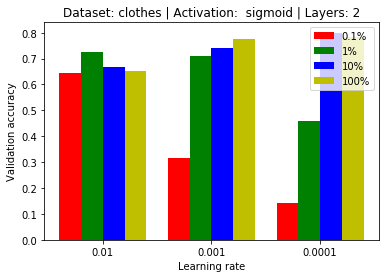
\includegraphics[scale=0.5]{accuracy_reduction_00.png}
            \caption{Validation accuracy comparison for the clothes dataset. The configuration with two fully connected layers and Sigmoid activations allows the highest accuracy for the smallest size of the dataset.}
            \label{fig:tf_clot}
        \end{center}
    \vskip -5mm
\end{figure*}

\begin{figure*}[tb]
    \vskip 5mm
        \begin{center}
            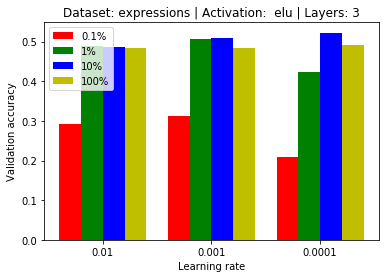
\includegraphics[scale=0.5]{accuracy_reduction_01.png}
            \caption{Validation accuracy comparison for the expression dataset. The configuration with three fully connected layers and ELU activations allows the highest accuracy for the smallest size of the dataset.}
            \label{fig:tf_exp}
        \end{center}
    \vskip -5mm
\end{figure*}

For each dataset, the configuration that provides the highest accuracy for the smallest dataset size are quite different, as seen in \ref{tab:tf_1}. It is specially important to note the activation functions. It is expected that the Sigmoid activation function gives better results since the uniform initialisation strategy is meant to benefit this activation function. However, in the case of expressions dataset, the best result is obtained with ELU, but the best accuracy using Sigmoid activations is not that far (0.30).

\begin{table*}[!htb]
  \centering
  \begin{tabular}{| l | l | l | l | l |}
    \hline
    \textbf{Dataset} & \textbf{Validation accuracy} & \textbf{Fully connected layers}& \textbf{Activation} & \textbf{Learning rates}\\ \hline
    Clothes & 0.64 & 2 & Sigmoid & 0.01 \\ \hline
    Expressions & 0.31  & 3 & ELU & 0.001 \\ \hline
  \end{tabular}
  \caption{Configuration that allows the highest accuracy for size of 0.1\% for clothes and expressions datasets}
  \label{tab:tf_1}
\end{table*}

The proposed approach has provided more benefits to the clothes dataset than to the expressions one, as seen in Figure \ref{fig:tf_clot} and Figure \ref{fig:tf_exp}. This gives us some clues about the complexity of the images in every dataset. Based on these results, it is possible to the expressions dataset was more challenging than the clothes dataset. 

In comparison with the baseline system, it is clearly evident that the performance of the proposed system is better. For the clothes dataset reaches a performance similar to the one obtained using data augmentation. However, for the expressions dataset, the performance surpasses the one obtained with data augmentation. This might indicate that the conversion from the original feature space (pixel intensity) to the feature space provided by VGG16 is more beneficial for the expressions than for the clothes.

\begin{table*}[!htb]
  \centering
  \begin{tabular}{| l | l | l | l | l |}
    \hline
    \textbf{Dataset} & \textbf{Baseline} & \textbf{Data Augmentation}& \textbf{Transfer learning} \\ \hline
    Clothes & 0.50 & 0.76 & 0.75 \\ \hline
    Expressions & 0.32  & 0.44 & 0.50 \\ \hline
  \end{tabular}
  \caption{Validation accuracy comparison between baseline system and approaches using data augmentation and transfer learning for size of 1\% for clothes and expressions datasets}
  \label{tab:tf_2}
\end{table*}

\subsubsection{\textbf{Interpretation and Discussion}}

[[TODO: Tidy This Up]]

Observing the behaviour of the fully connected layers for the smallest sizes of both datasets, it is evident that the system is more stable for the clothes than for the expressions as seen in figure behaviour.png In the case of the clothes, for 1\% and 0.1\% of the original size, the system reaches a point where it starts to overfit. However, it is noticeable how the configuration of the system is robust enough to try to minimise this situation. The history is different for the expressions. Here, the behaviour is completely different not just compared to the clothes, but between the sizes of the dataset. In the case of the 1\% of the size, the configuration of the system is not robust enough to minimise the effect of overfitting. Once the overfitting starts, the system cannot make too much about it. However, for the case of 0.1\%, the configuration of the system is robust, not just to minimise the effects of overfitting, but to recover from it. This is not something immediate and it takes some time.

\subsection{Siamese Neural Network}

\subsubsection{\textbf{Description and motivation}}

Our model consists of first 19 layers in VGG16 followed by a flatten layer which converts all features from the previous layers to
an equivalent n-dimensional matrix (n,) in python. These vectors are then passed to a fully connected layer with sigmoid activation which outputs 4096 vectors. Next, we pass these vectors to our defined L1 distance layer which calculates the L1 distance between pairs of input images as a number. Finally, we output the probability of each pair of images being in the same class based on a last fully connected layer, also with a sigmoid activation. Binary cross-entropy is therefore used as the loss function.

To avoid overfitting, we utilise L2 regularization with $\lambda=0.0001$. Since the original paper used different and decaying learning rates in each layer, adopting such approach on VGG16 would be difficult. We therefore simplified to use the Adam learning rule with a learning rate 0.001 as we have observed that choices of learning rate doesn't seem to affect much on the prediction accuracy.

\subsubsection{\textbf{Experimental setup}}

The goal is to train our VGG16-augmented Siamese Network to classify unseen classes of images by learning to distinguish similarity between images. The input is in terms of N pairs of image each having (64,64,3) matrix encoded as pixels. As in the original paper, each of the two twin images in every pairs of images are passed to the model separately with weight sharing. This is to ensure symmetric invariance in model, that is to ensure that L1 distance layer output the same distance when the order of the two twins image inputted is changed. This is done by defining the L1 distance layer $|x[first_twin] - x[second_twin]|$ where $x$ is the flattened output from VGG16 and input of the entire network takes the form $pairs=[first_twin,second_twin]$. First twin and second twin has input shape (batch_size,64,64,3). The batch size determines no. of pairs to be trained during each epoch. As suggested in the original paper, we also ensure 50$\%$ of same and different class are used in pairs and randomly sampled among $k$ available images in each classes. For the training data, we used first three catagories of animated facial expression dataset(42k images in 7 classes) and japanese female facial expression dataset (203 in 7 classes) in two separate runs. Both of the dataset also contains 7 classes of expression.

In the first approach, both training and test data are animated facial expression dataset. However, we only included the first three catagories during training and the 4 unseen class during test time. This is to test the effectiveness of the proposed model on predicting unseen images but with a softer restriction. The model is allowed to learn representation on subset of classes of the target dataset but tested on other unseen classes of the same dataset. Note that this approach is still distinct from standard machine learning procedure as training is not directly on same kind of target dataset. Among the three catagories, we randomly sampled 36 pairs of images randomly sampled from 900x3 available images from 3 classes in each epoch training. It is also ensured that 50$\%$ same and different classes are drawn.

In the second approach, restriction is increased and allow only related but entirely different dataset (Japanese female dataset) for 
training. There are in total 29x7 images in 7 catagories. Apparently, the size of dataset is so few comparing to dataset in first
approach. The reason of using this dataset is due to limited availability of grayscale facial expression dataset from internet and this is the only dataset that shares most geometric similarity with the target set(animated facial expression), as location ,classes and placement angles are most similar comparing to other datasets such as extended cohn-kanade facial dataset.

[[PLACEHOLDER]]

\subsubsection{\textbf{Results}}

In the first approach, training accuracy increases for first 50 epoch training ranging from $49-68\%$ which proves that the model is in fact learning. During test time, 320 one shot learning tasks is performed after epochs of training. In each one shot learning task,6 different and 1 same class pairs of image is randomly drawn from 6000x4 images. If the model successfully predicts the pair, we add one to accuracy, the overall accuracy is then calculated in terms of $100.0*n_correct / 320$. At 1st epoch, accuracy is around $28\%$ which is close to random guessing. At 20th epoch, accuracy reaches $40-49\%$ and doesnt improve further for more epochs. In second approach, we used 96 and 198 batch_size in training to allows more learning and test if overfitting would occur. Moreover,similar 320 one shot learning tasks are performed to classify 7 unseen catagories from pairs randomly drawn from 6000x7 images. For 96 batch size after 50th epoch of training. Test accuracy ranges from $22.8125-28.4375\%$. For 198 batch size, test accuracy falls in range of $20-30\%$.

\subsubsection{\textbf{Interpretation and Discussion}}

For the first approach, we achieved best test accuracy of $50\%$. This might be because training set shares generic features on hairstyle,shape of face, sexuality of characters with target set. However, the result also showed effectiveness of using similarity differences to classify unseen images as we have not trained the network to learn about the other 4 expressions.

Note that in both of the approaches, test accuracy is better than random guessing by $~100\%$ which suggests our model is in fact working. In the second approach, test accuracy drops significantly which is probably due to insufficient training set. Moreover, there are greater differences between training and target set than in first approach. Given more available dataset and time, it is expected that the second approach would perform better. Another reason of the performances could be attributed to use of grayscale images. Since VGG16 trained on RGB images, weights in the network are trained to learn colorful images. Using grayscale images would alter performances of VGG16. Overall, results have shown that our model demonstrated the ability to predict unseen images by transferring representation of related but different images to solve one shot learning tasks, to preliminary extent. 

\section{Related work}
\label{sec:related}

In order to place our research in a wider context, we offer a brief review of published work that that has been foundational in our efforts to explore the implications of using small data on convolutional neural networks. Initially, our research associated with small data was inspired by a quote from Andrew Ng from an article on nanonets \cite{nanoNets}.

\begin{displayquote}
I think AI is akin to building a rocket ship. You need a huge engine and a lot of fuel. If you have a large engine and a tiny amount of fuel, you won’t make it to orbit. If you have a tiny engine and a ton of fuel, you can’t even lift off. To build a rocket you need a huge engine and a lot of fuel. The analogy to deep learning is that the rocket engine is the deep learning models and the fuel is the huge amounts of data we can feed to these algorithms.
\end{displayquote}

Further, understanding how much data one may require to obtain a satisfactory level of performance on image classification problems seemed to be an interesting proposition \cite{howMuchData}.

As a result, a review of the literature within the domain of transfer learning was performed. An overview of this technique is provided within the introduction to this report \ref{sec:intro}, however we reviewed papers such as \cite{NIPS2014_5347} and \cite{oquab2014learning}. We found that transfer learning is a fairly versitile method to reduce training time and data required, especially when dealing with low level representations \cite{NIPS2014_5347}. As we can demonstrate that small data may be an issue in image classification tasks that utilise convolutional neural networks \cite{interim-report}, we also thought it would be interesting to investigate how distinctly different (but comparable) datasets (with a large difference between the degrees of perceived visual similarity between classes) perform agaisnt one another in image classification tasks that utilise transfer learning. This in and of itself is an interesting research domain because the notion of perceived visual similarity has only recently began being explored within the literature. Consequently, we decided to consider methods by which we could compute similarity metrics for measuring the difference between classes and datasets. As one-shot learning tasks, such as person re-identification \cite{ahmed2015improved} performs similar roles (by passing some similarity metric through a threshold function), we began to explore the literature related to siamese convolutional networks \cite{koch}.

Any future work would likely build upon the aforementioned apporach to measuring perceived visual similarity between datasets and the effect that this has on positive and negative transfer.

\section{Conclusions}
\label{sec:conclusions}

Siamese part conclusion:Overall, the results demonstrated the capability of our model on classifying unseen classes (one shot learning) to a certain extent using learnt representations from related data to distinguish similarity.

This is particularly important as a lot of data (e.g. minorities language, images of rare disease )are insufficient for training in reality. These experiment motivated the use of transfer learning on solving insufficient training set and provided some preliminary 

results of transfer learning on image recognition. Moreover, these research questions could support more advanced researches.

%\bibliographystyle{abbrv}
\bibliography{biblo.bib}

\end{document}
